\documentclass{standalone}
\usepackage{tikz}
\usetikzlibrary{shapes.geometric, arrows.meta, positioning}

% Define styles for nodes
\tikzset{
    block/.style={draw, minimum width=2cm, minimum height=1cm, align=center},
    amplifier/.style={trapezium, trapezium left angle=60, trapezium right angle=120, draw, fill=black!80, text=white, minimum width=1.5cm, minimum height=1.5cm},
    beamsplitter/.style={rectangle, draw, fill=black!80, text=white, minimum width=1cm, minimum height=3cm},
    arrow/.style={-{Stealth[scale=1.2]}},
    label/.style={font=\scriptsize}
}

\begin{document}
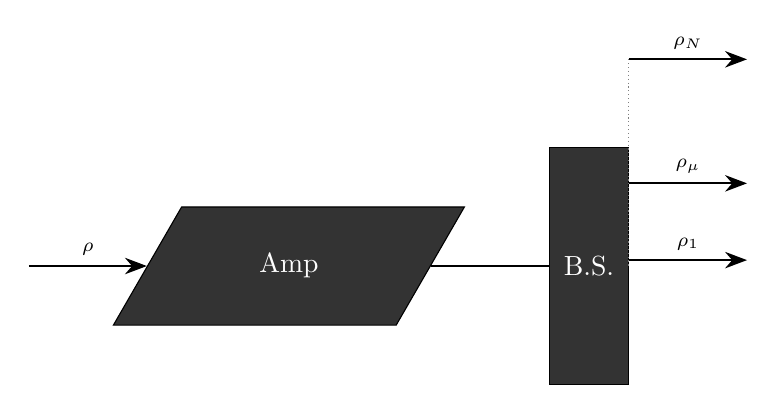
\begin{tikzpicture}[node distance=1.5cm]

% Draw the amplifier
\node [amplifier] (amp) {Amp};

% Draw the beam splitter
\node [beamsplitter, right=of amp] (bs) {B.S.};

% Draw input arrow and label
\draw [arrow, thick] ([xshift=-1.5cm]amp.west) -- (amp.west) node [midway, above, label] {$\rho$};

% Draw output arrows and labels
\foreach \i/\label [count=\j from 1] in {0.075/\rho_1, 0.4/\rho_\mu, 0.925/\rho_N} {
    \draw [arrow, thick] ([yshift=\i*3cm-0.15cm]bs.east) -- ++(1.5cm,0) node [midway, above, label] {$\label$};
    \draw [densely dotted, gray] ([yshift=\i*3cm-0.15cm]bs.east) -- (bs.east);
}

% Draw connection between amplifier and beam splitter
\draw [thick] (amp.east) -- (bs.west);

\end{tikzpicture}
\end{document}